\chapter{Lukuteorian tuloksia}

%Tässä luvussa käsitellään joitakin lukuteorian tunnetuimpia tuloksia ja niiden todistuksia.

\section{Suurin yhteinen tekijä ja Eukleideen algoritmi}
Seuraavaksi käsitellään kahden positiivisen kokonaisluvun yhteisiä tekijöitä ja esitetään käytännöllinen menetelmä {\em suurimman yhteisen tekijän} etsimiseksi.

\subsection*{Tutkimustehtävä}
\begin{enumerate}
\item Määritä lukujen $45$ ja $75$ kaikki positiiviset tekijät.
\item Mitkä ovat lukujen yhteiset positiiviset tekijät?
\item Mikä on lukujen suurin yhteinen tekijä?
\item Supista murtoluku $\frac{45}{75}$.
\end{enumerate}

\begin{esimerkki}
%{\bf Esimerkki 1.}
Määritä lukujen $30$ ja $84$ kaikki positiiviset tekijät. Mitkä ovat niiden yhteiset positiiviset tekijät? Mikä on niiden suurin yhteinen tekijä?

{\bf Ratkaisu:} Luvun $30$ positiiviset tekijät ovat $1, 2, 3, 5, 6, 10, 15$ ja $30$. Luvun $84$ positiiviset tekijät ovat $1, 2, 3, 4, 6, 7, 12, 14, 21, 28, 42$ ja $84$.

Lukujen $30$ ja $84$ yhteiset positiiviset tekijät ovat $1, 2, 3$ ja $6$. Yhteisistä tekijöistä suurin on $6$.

{\bf Vastaus:} 
Yhteiset positiiviset tekijät ovat $1, 2, 3$ ja $6$. Suurin yhteinen tekijä on $6$.
\end{esimerkki}

%\fbox{
\laatikko{
\begin{minipage}{12cm}
{\bf Suurin yhteinen tekijä.}
%\medskip
%---
%{\bf Teorialaatikko [Suurin yhteinen tekijä]}
Olkoot $a$ ja $b$ positiivisia kokonaislukuja. Positiivista kokonaislukua $d$ sanotaan lukujen $a$ ja $b$  suurimmaksi yhteiseksi tekijäksi, jos seuraavat ehdot ovat voimassa:
\begin{enumerate}
\item Luku $d$ on lukujen $a$ ja $b$ tekijä, eli $d| a$ ja $d | b$. 
\item Luku $d$ on suurin lukujen $a$ ja $b$ tekijöistä.
\end{enumerate}
Lukujen $a$ ja $b$ suurinta yhteistä tekijää merkitään $\syt(a,b)$ tai joskus $\gcd(a,b)$. Lyhenne gcd tulee englanninkielisestä ilmaisusta {\em greatest common divisor}.
%---
\end{minipage}
}

Kahden luvun suurin yhteinen tekijä voidaan ainakin periaatteessa aina löytää luettelemalla näiden lukujen tekijät, etsimällä lukujen yhteiset tekijät ja valitsemalla lopuksi yhteisistä tekijöistä suurin. Tämä menettelytapa muuttuu kuitenkin hankalaksi suurten lukujen kohdalla, vaikka käytössä olisi tietokone.

Tehokkaan algoritmin suurimman yhteisen tekijän etsimiseksi esitti aleksandrialainen matemaatikko Eukleides (n. 300 eaa.) teoksessaan Stoikheia (Alkeet, latinaksi Elementa). Alkeet on yksi matematiikan historian tärkeimmistä teoksista, ja se säilyi käytetyimpänä geometrian oppikirjana aina 1800-luvulle saakka. Teoksessa esitettyä algoritmia kutsutaan {\em Eukleideen algoritmiksi}, ja se perustuu seuraavaan lemmaan:

%{\bf Lause (Jaollisuuden peruslause, s.108 / Pitkä matematiikka)}

\laatikko{
%\begin{minipage}{12cm}
{\bf Lemma.} Olkoot $a$ ja $b$ sellaisia positiivisia kokonaislukuja, että
\[
a=qb+r,
\]
missä $q$ sekä $r$ ovat kokonaislukuja ja $0<r<b$. Tällöin kokonaisluku\newline $c$ on lukujen $a$ ja $b$ yhteinen tekijä, jos ja vain jos $c$ on lukujen $b$ ja $r$\newline yhteinen tekijä.
%\end{minipage}
}

\begin{todistus}
Oletetaan aluksi, että $c$ on jokin lukujen $a$ ja $b$ yhteinen tekijä. Osoitetaan, että se on myös lukujen $b$ ja $r$ yhteinen tekijä.

Kirjoitetaan $r=a-qb$. Luvun $c$ täytyy olla luvun $r$ tekijä, koska se on lukujen $a$ ja $b$ tekijä. Siten $c$ on lukujen $b$ ja $r$ yhteinen tekijä.

Oletetaan, että $c$ on jokin lukujen $b$ ja $r$ yhteinen tekijä. Koska $a=qb+r$, luvun $c$ täytyy olla myös luvun $a$ tekijä. Siten $c$ on lukujen $a$ ja $b$ yhteinen tekijä.

\end{todistus}

\laatikko{
\begin{minipage}{12cm}
{\bf Seuraus.} Jos $a$ ja $b$ ovat positiivisia kokonaislukija ja $a=qb+r$, missä $q$ sekä $r$ ovat kokonaislukija ja $0<r<b$, niin $\syt(a,b)=\syt(b,r)$.
\end{minipage}
}

\begin{todistus}
Lemman perusteella lukujen $a$ ja $b$ yhteiset tekijät ovat samat kuin lukujen $b$ ja $r$ yhteiset tekijät. Erityisesti siis lukujen $a$ ja $b$ suurimman yhteisen tekijän täytyy olla sama kuin lukujen $b$ ja $r$ suurimman yhteisen tekijän.
\end{todistus}

%{\bf ... täydennä}


Eukleideen algoritmin idea on seuraava: Lähdetään liikkeelle kahdesta positiivisesta kokonaisluvusta $a$ ja $b$, $a\ge b$, joiden yhteistä tekijää etsitään. Ensimmäinen askel on esittää luku $a$ luvun $b$ avulla jakoyhtälönä:
\[
a=q_1b + r_1, \qquad 0 \le r_1 < b.
\]

Jos jakojäännös $r_1=0$, niin $b|a$ ja $\syt(a,b)=b$. Jos $r_1\neq 0$, jaetaan $b$ luvulla $r_1$, jolloin saadaan esitys
\[
b= q_2r_1+r_2, \qquad 0 \le r_2 < r_1,
\]
missä $q_2$ on jakolaskun $b/r_1$ osamäärä ja $r_2$ jakojäännös.

Jos $r_2=0$, niin $r_1$ on suurin yhteinen tekijä ja voidaan lopettaa. Mikäli näin ei ole, jatketaan jakamalla luku $r_1$ luvulla $r_2$, jolloin saadaan
\[
r_1 = q_3r_2 + r_3, \qquad 0 \le r_3 < r_2.
\]

Näin jatkamalla päädytään lopulta jakolaskuun, joka menee tasan. Lukujen $a$ ja $b$ suurin yhteinen tekijä on viimeinen nollasta eroava jakojäännös. Koska algoritmissa esiintyy laskeva jono $b>r_1>r_2> \cdots \ge 0$, tarvitaan enintään $b$ askelta. Algoritmissa tarvittavat jakolaskut kannattaa yleensä tehdä laskimella.

\begin{esimerkki}
%{\bf Esimerkki 2.}
Määritä $\syt(84, 30)$ Eukleideen
algoritmia käyttäen.

{\bf Ratkaisu:}

\begin{tabular}{lcl}
$84 = 2 \cdot 30 + 24$ & &
Jaetaan luku 84 luvulla 30 ja esitetään luku 84 luvun 30
\\
&& avulla. Jakojäännös ei ole nolla.\\
$30 = 1 \cdot 24 + 6$ & & Jaetaan luku 30 saadulla
jakojäännöksellä 24 ja \\
&& esitetään luku 30 luvun 24 avulla. Jakojäännös ei \\
&& ole nolla. \\
$24 = 4 \cdot 6$ & & Esitetään luku 24 jakojäännöksen 6
avulla. Nyt jako \\
&& menee tasan.
\end{tabular}

(Kuvioon tulee nuolet luvusta 30 lukuun 30 ja luvusta 24
lukuun 24, sekä luvusta 24
lukuun 24 ja luvusta 6 lukuun 6.)

Suurin yhteinen tekijä on viimeinen nollasta eroava
jakojäännös, $6$. Siis $\syt(84, 30) = 6$. Saatiin sama
tulos kuin esimerkissä 1.

{\bf Vastaus:} $\syt(84, 30) = 6$.
\end{esimerkki}

\begin{esimerkki}
%{\bf Esimerkki 3.}
Määritä $\syt(16515,3951)$ Eukleideen
algoritmia käyttäen.

{\bf Ratkaisu:}
Eukleideen algoritmi johtaa yhtälöihin:
\[
16515 = 4 \cdot 3951 + 711,
\]
\[
3951 = 5 \cdot 711 + 396,
\]
\[
711 = 1 \cdot 396 + 315,
\]
\[
396 = 1 \cdot 315 + 81,
\]
\[
315 = 3 \cdot 81 + 72,
\]
\[
81 = 1 \cdot 72 + 9,
\]
\[
72 = 8 \cdot 9.
\]
Suurin yhteinen tekijä on viimeinen nollasta eroava
jakojäännös, siis tässä tapauksessa $9$. Siten
\[
\syt(16515,3951) = 9.
\]

{\bf Vastaus:} $\syt(16515, 3951) = 9$.
\end{esimerkki}

%\newpage

%\section*{Tehtäviä}

\Harjoitustehtavat

\begin{enumerate}

\item Määritä lukujen suurin yhteinen tekijä.
\begin{itemize}
\item[a)] $15$ ja $20$
\item[b)] $9$ ja $36$
\item[c)] $4$ ja $7$
\end{itemize}

\item Määritä Eukleideen algoritmia käyttäen
\begin{itemize}
\item[a)] $\syt(184,152)$
\item[b)] $\syt(227,143)$.
\end{itemize}

\item Määritä Eukleideen algoritmia käyttäen
\begin{itemize}
\item[a)] $\syt(272,1479)$
\item[b)] $\syt(4719,18207)$.
\end{itemize}

\item Esitä murtoluku  a) $\frac{143}{605}$  b) $\frac{5989}{30899}$  supistetussa muodossa. Vihje: Määritä osoittajan ja nimittäjän suurin yhteinen tekijä.

\item Osoita, että murtoluku $\frac{8788}{13475}$ ei supistu.

\item Leirille osallistui 780 tyttöä ja 612 poikaa. Osallistujat jaettiin keskenään yhtä suuriin ryhmiin siten, että kussakin ryhmässä oli vain tyttöjä tai poikia. Mikä oli suurin mahdollinen ryhmäkoko?

\item
Määritä lukujen $188\, 000\, 100$ ja $188$ suurin yhteinen tekijä.

\item Olkoon $a$ positiivinen kokonaisluku. Määritä
\begin{itemize}
\item[a)] $\syt(a,a)$
\item[b)] $\syt(a,1)$
\item[c)] $\syt(a^2,a)$
\item[d)] $\syt((a+1)!,a!)$.
\end{itemize}
Merkintä $a!$ tarkoittaa luvun $a$ {\em kertomaa}. Se on tulo $a! = a \cdot (a-1) \cdot (a-2) \cdot \ldots \cdot 3 \cdot 2 \cdot 1$.

\item Olkoon $n$ positiivinen kokonaisluku. Osoita Eukleideen algoritmia käyttäen, että $\syt(n+1,n)=1$.

\item Olkoon $n$ positiivinen kokonaisluku. Määritä lukujen $n^2 + 2n$ ja $n + 1$ suurin yhteinen tekijä.

\item Olkoon $n$ positiivinen kokonaisluku. Osoita, että $\syt(3^{n+1} + 10,3^n + 2)=1$.

\end{enumerate}


{\bf Kotitehtäviä}

\begin{enumerate}

\item Määritä lukujen suurin yhteinen tekijä.
\begin{itemize}
\item[a)] $63$ ja $7$
\item[b)] $64$ ja $33$
\item[c)] $45$ ja $60$
\end{itemize}

\item Määritä Eukleideen algoritmia käyttäen
\begin{itemize}
\item[a)] $\syt(657,306)$
\item[b)] $\syt(2197,4641)$
\item[c)] $\syt(15787,4111)$.
\end{itemize}

\item
Esitä murtoluku  a) $\frac{182}{299}$  b) $\frac{7697}{32041}$  supistetussa muodossa.

\item Leipomo suljettiin remontin ajaksi. Ennen sulkemista laskettiin, että leipomon varastossa oli 4896 vehnäsämpylää ja 1408 grahamsämpylää. Sämpylät pakattiin kuljetusta varten keskenään samankokoisiin pusseihin siten, että kuhunkin pussiin tuli vain vehnä- tai grahamsämpylöitä. Mikä oli suurin mahdollinen pussikoko? Oletetaan, että vehnäsämpylä oli samankokoinen kuin grahamsämpylä ja että yksikään pussi ei jäänyt vajaaksi.

\item Määritä lukujen $468\, 468\, 468\, 108$ ja $234$ suurin yhteinen tekijä.

\item Olkoot $a$, $b$ ja $c$ positiivisia kokonaislukuja. Lukujen $a$, $b$ ja $c$ suurin yhteinen tekijä eli $\syt(a,b,c)$ voidaan määrittää siten, että ensin määritetään kahden luvun suurin yhteinen tekijä ja sitten tämän ja kolmannen luvun suurin yhteinen tekijä. Määritä
\begin{itemize}
\item[a)] $\syt(15,30,40)$
\item[b)] $\syt(6,9,11)$
\item[c)] $\syt(171,456,665)$.
\end{itemize}

\item Olkoot $a$ ja $b$ positiivisia kokonaislukuja ja $\syt(a,b)=9$. Voiko tällöin yhtälö $a + b = 186$ olla tosi?

\item Olkoon $n$ positiivinen kokonaisluku. Tutki, mitä arvoja $\syt(n+4,n)$ voi saada.

\item Olkoon $n$ positiivinen kokonaisluku. Määritä lukujen $n^2 + 3n$ ja $n + 2$ suurin yhteinen tekijä.

\item Olkoot $a$ ja $b$ positiivisia kokonaislukuja. Osoita, että $\syt(a,b)$ on jaollinen kaikilla lukujen $a$ ja $b$ yhteisillä tekijöillä.

\end{enumerate}


\newpage

\section{Diofantoksen yhtälöt}
Noin vuoden 250 tienoilla elänyt Diofantos oli yksi viimeisistä antiikin Aleksandriassa vaikuttaneista suurista matemaatikoista. Aleksandrian suuruuden ajan oppineisuuden keskuksena katsotaan yleisesti päättyneen noin sata vuotta myöhemmin pakanaksi ja noidaksi syytetyn naismatemaatikko Hypatian murhaan vuonna 415. Vaikka Diofantos kirjoitti kreikaksi ja häntä usein kutsutaan kreikkalaiseksi matemaatikoksi, Diofantos oli todennäköisesti kreikkalaistunut babylonialainen. 

\subsection*{Tutkimustehtävä}
\begin{enumerate}
\item Missä sijaitsevat ne $xy$-tason pisteet, joiden koordinaatit toteuttavat yhtälön $x + 3y = 6$?
\item Etsitään seuraavaksi kokonaislukuratkaisuja kahden muuttujan yhtälölle $x + 3y = 6$. Määritä yhtälölle jokin kokonaislukuratkaisu.
\item Määritä yhtälölle vielä ainakin kolme muuta kokonaislukuratkaisua. Kuinka monta ratkaisua yhtälöllä on kaiken kaikkiaan?
\item Määritä kaikki yhtälön $x + 3y = 6$ kokonaislukuratkaisut.
\item Keksi vastaava kokonaislukukertoiminen kahden muuttujan yhtälö, jolla ei ole yhtään kokonaislukuratkaisua.
\end{enumerate}

%{\bf Marginaaliin:}
Diofantoksesta ei tiedetä kovinkaan paljon, mutta hänen tarkka \hbox{elin}\-ikän\-sä tunnetaan kuitenkin hautakiveen ikuistetusta matemaattisesta ongelmasta: Diofantoksen poikavuodet kestivät $1/6$ hänen elämästään, parta alkoi kasvaa $1/12$ tämän jälkeen, $1/7$ kuluttua hän meni naimisiin ja hänen poikansa syntyi $5$ vuotta myöhemmin. Poika eli puolet siitä, mitä isänsä, ja isä kuoli neljä vuotta poikansa kuoleman jälkeen. Ongelma johtaa yhtälöön
\[
\frac{1}{6}x + \frac{1}{12} x + \frac{1}{7}x + 5 + \frac{1}{2}x+ 4=x,
\]
josta Diofantoksen elinvuodet voidaan ratkaista. Ratkaisu on $x=84$.

{\em Diofantoksen yhtälöiksi} kutsutaan muotoa
\[
ax + by = c
\]
olevia yhtälöitä, missä $x$ ja $y$ ovat kokonaislukuja. Yhtälössä esiintyvät vakiot $a,b$ ja $c$ ovat myös kokonaislukuja ja ainakin toinen luvuista $a,b$ on nollasta poikkeava. 
Tässä kurssissa käsitellään vain kyseistä muotoa olevia yhtälöitä, mutta nykyään matematiikassa sanotaan Diofantoksen yhtälöiksi myös muita yhtälöitä, joissa ratkaistavana on yksi tai useampi kokonaisluku. Diofantos ei itse tutkinut tällaisia yhtälöitä.

Diofantoksen yhtälöllä voi olla useita ratkaisuja tai ei yhtään ratkaisua. Esimerkiksi
yhtälölle
\[
3x + 6 y = 18
\]
voidaan löytää ainakin seuraavat ratkaisut:
\[
18 = 3\cdot 4 + 6\cdot 1 = 3\cdot (-6)+6\cdot 6 = 3\cdot10 + 6\cdot (-2).
\]
Toisaalta esimerkiksi yhtälöllä $2x+10 y =17$ ei ole ratkaisua.

Ratkaisujen etsimisessä on hyötyä tiedosta, että jos on annettu positiiviset kokonaisluvut $a$ ja $b$, niin on aina olemassa kokonaisluvut $x$ ja $y$ siten, että
%positiivisille kokonaisluvuille $a,b$ on aina olemassa kokonaisluvut $x$ ja $y$, joille
\[
\syt(a,b) = ax + by.
\]
Käytännössä kertoimien etsiminen ei ole vaikeaa, sillä siinä voidaan käyttää hyväksi Eukleideen algoritmia.
% Tästä esitysmuodosta ja Eukleideen algoritmista hyötyä Diofantoksen yhtälöiden ratkaisemisessa.

\begin{esimerkki}
%{\bf Esimerkki 1.}
Ratkaise Diofantoksen yhtälö
$\syt(84,30) = 84x + 30y$.

{\bf Ratkaisu:} Lukujen $84$ ja $30$ suurin yhteinen tekijä
ratkaistiin edellisen kappaleen esimerkissä 2. Eukleideen
algoritmi johti yhtälöihin
\begin{eqnarray*}
84 &=& 2 \cdot 30 + 24,\\
30 &=& 1 \cdot 24 + 6,\\
24 &=& 4 \cdot 6,
\end{eqnarray*}
joten $\syt(84,30) = 6$. Ratkaistavana on siis yhtälö $6
= 84x + 30y$.

Pyritään nyt ilmaisemaan luku 6 lukujen 84 ja 30 avulla.
Kuljetaan Eukleideen algoritmia lopusta alkuun ja
ratkaistaan jakoyhtälöistä jakojäännökset. Viimeinen
nollasta eroava jakojäännös on $6$. Lausutaan se lukujen
$30$ ja $24$ avulla: $6 = 30 - 1 \cdot 24$. Saadussa
lausekkeessa luku $24$ on edellisen yhtälön jakojäännös,
joka puolestaan voidaan lausua lukujen $84$ ja $30$
avulla: $24 = 84 - 2 \cdot 30$. Yhdistämällä tulokset
saadaan luku $6$ ilmaistua lukujen $84$ ja $30$ avulla:
\[
6 = 30 - 1 \cdot 24 = 30 - 1 \cdot (84 - 2 \cdot 30) = 30
- 1 \cdot 84 + 2 \cdot 30 = -1 \cdot 84 + 3 \cdot 30.
\]
Siis $6 = 84 \cdot (-1) + 30 \cdot 3$, joten yhtälön $6=84x+30y$
ratkaisu on $x = -1$ ja $y = 3$.

{\bf Vastaus:} $x = -1$ ja $y = 3$.
 %Samat luvut kuin edellisen kappaleen esimerkissä 2.
\end{esimerkki}

Diofantoksen yhtälöitä voidaan usein ratkaista esimerkiksi tietokoneella, mutta se onnistuu myös seuraavaa tulosta käyttämällä.

\laatikko{
{\bf Lause.} Diofantoksen yhtälöllä
\[
a x + b y = c
\]
on ratkaisu, jos ja vain jos $d|c$, kun $d=\syt(a,b)$.
}

\begin{todistus}
%{\bf Mieti todistuksen muotoilua, vars. jos ja vain jos.}
%Jaa kahteen osaan, ensin toiseen ja sitten toiseen suuntaan. Oletukset eksplisiittisesti.

Osoitetaan aluksi epäsuoraa todistusta käyttämällä, että ratkaisun olemassaolosta seuraa $d|c$. Tehdään vastaoletus, että $d \nmid c$. Tällöin yhtälöllä ei voi olla ratkaisua, koska $d|a$ ja $d|b$, joten $d$ jakaa yhtälön vasemman puolen mutta ei oikeaa puolta.

On vielä osoitettava ekvivalenssiväitteen toinen suunta: Jos $d|c$, niin kyseisellä Diofantoksen yhtälöllä on ratkaisu. Jos $d|c$, niin $c=dt$ jollakin kokonaisluvulla $t$. Aikaisemmin todettiin, että lukujen $a$ ja $b$ suurin yhteinen tekijä voidaan kirjoittaa muodossa
\[
d=\syt(a,b)=a x_1 + b y_1
\]
joillekin luvuille $x_1$ ja $y_1$. Koska
\[
c = dt = (ax_1 + by_1)t = a(tx_1)+ b(ty_1),
\]
saadaan pari $x=tx_1$ ja $y=ty_1$, joka toteuttaa alkuperäisen yhtälön.
\end{todistus}

\laatikko{
\begin{minipage}{12cm}
{\bf Lause.}
Jos
\[
a x + b y = c
\]
on ratkeava Diofantoksen yhtälö, sen yksi ratkaisu on $x=tx_1$ ja $y=ty_1$, missä kertoimet $x_1$ ja $y_1$ määräytyvät yhtälöstä
\[
d=\syt(a,b)=a x_1 + b y_1 \textrm{ ja } t=c/d.
\]
\end{minipage}
}

\begin{todistus}
Edellisen lauseen nojalla Diofantoksen yhtälöllä
\[
d= a x + b y,
\]
missä $d=\syt(a,b)$, on ratkaisu. Merkitään jotakin kyseisen yhtälön ratkaisua $x_1,y_1$.

On osoitettava, että tämän ratkaisun avulla voidaan löytää haluttua muotoa oleva ratkaisu alkuperäiselle yhtälölle
\[
a x + b y = c.
\]
Edellisen lauseen perusteella Diofantoksen yhtälöllä on ratkaisu, jos ja vain jos $d|c$. Siten $t=c/d$ on kokonaisluku.

Kerrotaan yhtälön
\[
d= a x_1 + b y_1
\]
molemmat puolet luvulla $t=c/d$. Tällöin saadaan
\[
c=td=t(a x_1 + b y_1) = a(tx_1)+ b(ty_1).
\]
Tämä osoittaa, että $x=tx_1$ ja $y=ty_1$ on alkuperäisen Diofantoksen yhtälön ratkaisu.
\end{todistus}

Itse asiassa jos $x_0$ ja $y_0$ ovat yhtälön $ax + by = c$ jokin ratkaisu, niin sen kaikki ratkaisut saadaan kaavoista
\[
x= x_0 + n\frac{b}{d}, \textrm{ ja } y=y_0 - n\frac{a}{d}, \textrm{ missä } \qquad n\in\mathbb{Z} \textrm{ ja } d=\syt(a,b).
\]
Erityisesti siis jokaisella ratkeavalla Diofantoksen yhtälöllä on äärettömän monta ratkaisua. Ratkaisussa esiintyvät kertoimet saattavat kuitenkin olla negatiivisia lukuja.

\begin{esimerkki}
%{\bf Esimerkki 2.}
Määritä Diofantoksen yhtälön
\[
172x + 20y = 1000
\]
jokin ratkaisu.

{\bf Ratkaisu:} Tutkitaan ensin, onko Diofantoksen yhtälöllä $172x + 20y = 1000$ ratkaisua. Määritetään $\syt(172,20)$ Eukleideen algoritmia käyttäen:
\[
172 = 8 \cdot 20 +12,
\]
\[
20 = 1\cdot 12 + 8,
\]
\[
12 = 1 \cdot 8 +4,
\]
\[
8=2\cdot 4.
\]
Siten $\syt(172,20)=4$. Koska $4|1000$, Diofantoksen yhtälöllä on ratkaisu.

Ratkaisun löytämiseksi täytyy esittää luku $4$ lukujen $172$ ja $20$ avulla muodossa 
\[
4=172\cdot x_1 + 20 \cdot y_1.
\]
Soveltamalla Eukleideen algoritmin askelia käänteisessä järjestyksessä saadaan
\begin{eqnarray*}
4 &=& 12 - 8\\
  &=& 12-(20-12) \\
  &=& 2\cdot 12-20 \\
  &=& 2 \cdot (172-8\cdot 20)-20 \\
  &=& 2\cdot 172 +(-17) \cdot 20.
\end{eqnarray*}
Kertomalla tämä lauseke luvulla $1000/4=250$ saadaan viimein
\begin{eqnarray*}
1000 = 250\cdot 4 &=& 250 \cdot (2\cdot 172 +(-17) \cdot 20) \\
 &=& 500\cdot 172 + (-4250) \cdot 20.
\end{eqnarray*}
Siten yhtälön $172x + 20y = 1000$ ratkaisu on $x=500$ ja $y=-4250$.

{\bf Vastaus:} $x=500$ ja $y=-4250$
\end{esimerkki}

\begin{esimerkki}
%{\bf Esimerkki 3.}
Määritä Diofantoksen yhtälön $172x + 20y = 1000$ kaikki
ratkaisut. Mitkä niistä toteuttavat ehdon $|x|+|y|\le
50$?

{\bf Ratkaisu:}
Diofantoksen yhtälön $ax+by=c$ kaikki ratkaisut saadaan
kaavoista
\[
x=x_0+n\frac{b}{d}\textrm{ ja }y=y_0-n\frac{a}{d},
\]
missä $x_0$ ja $y_0$ ovat yhtälön jokin ratkaisu,
$d=\syt(a,b)$ ja $n$ on mikä tahansa
kokonaisluku. Diofantoksen yhtälössä $172x+20y=1000$ on
$a=172$, $b=20$, ja edellisen
esimerkin nojalla $x_0=500$, $y_0=-4250$ ja $d=4$.
Sijoittamalla kaavoihin saadaan
yhtälön $172x+20y=1000$ ratkaisuiksi
\[
x=500+n\frac{20}{4}\textrm{ ja }y=-4250-n\frac{172}{4}
\]
eli $x=500+5n$ ja $y=-4250-43n$, $n\in\Z$.

Jotta ehto $|x| +|y|\le 50$ toteutuisi, pitää muuttujien
$x$ ja $y$ olla itseisarvoiltaan pieniä. Tutkitaan
yhtälöitä $x = 500 + 5n = 0$ ja $y = -4250 - 43n = 0$ ja
ratkaistaan kummastakin parametri $n$.
\begin{eqnarray*}
500 + 5n &=& 0\\
5n &=& -500\\
n &=& -100\\
-4250 - 43n &=& 0\\
-43n &=& 4250\\
n &\approx&-98,8
\end{eqnarray*}
Osoittautuu siis, että molempien yhtälöiden mukaan $n$
on lähellä arvoa $-100$ tai $-99$. Taulukoidaan myös
muutamia muita näitä arvoja lähellä olevia parametrin $n$
arvoja ja tutkitaan kussakin tapauksessa, toteutuuko ehto
$|x| + |y| \le 50$.

\begin{center}
\begin{tabular}{|c|c|c|c|}
\hline
$n$ & $x$ & $y$ & $|x|+|y|$ \\

\hline
$-97$&$15$&$-79$&$94$\\
\hline
$-98$&$10$&$-36$&$46$\\
\hline
$-99$&$5$&$7$&$12$\\
\hline
$-100$&$0$&$50$&$50$\\
\hline
$-101$&$-5$&$93$&$98$\\
\hline
$-102$&$-10$&$136$&$146$\\
\hline
\end{tabular}
\end{center}

Taulukosta nähdään, että $|x|+|y| \le 50$, kun $x = 10$
ja $y = -36$, kun $x = 5$ ja $y = 7$ tai kun $x = 0$ ja
$y = 50$. Muita ratkaisuja ei ole, sillä kun $n$ pienenee
tai suurenee taulukon arvoista, niin sekä $|x|$ että $|
y|$ suurenevat.

{\bf Vastaus:} Kaikki ratkaisut ovat  $x=500+5n$ ja $y=-4250-43n$, $n\in\Z$. Näistä ehdon $|x|+|y|\le 50$ toteuttavat ratkaisut $x = 10$ ja $y = -36$, $x = 5$ ja $y = 7$ sekä $x = 0$ ja $y = 50$.
\end{esimerkki}

\begin{esimerkki}
%{\bf Esimerkki 4.}
 (Kexleruksen viiniongelma)
%(Lisämateriaalia)
Suomen ensimmäinen matematiikan professori, Turun
akatemiassa vaikuttanut Simon Kexlerus (1602--1669) jätti
jälkeensä seuraavan ongelman.

\begin{center}
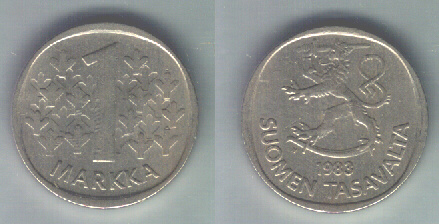
\includegraphics[width=4cm]{pictures/wikimarkka.jpg} % /NVI

Markan kolikko vuodelta 1983.
\end{center}

Sinulla on viinejä, jotka maksavat $3$, $5$, $8$ ja $10$
markkaa pullolta. Ota yhteensä kymmenen täyttä pulloa ja
tee niistä sekoitus, joka maksaa $6$ markkaa pullolta.
Kuinka monta pulloa kutakin viinilajia on otettava?

{\bf Ratkaisu:} Merkitään tarvittavien pullojen määrää
$a,b,c$ ja $d$. Ongelma johtaa kahteen Diofantoksen
yhtälöön,
\[
a+b+c+d = 10
\]
ja
\[
3a+5b+8c+10d = 60.
\]
Selvästi tehtävän ratkaisut ovat kokonaislukuja välillä
$0,\ldots,10$. Tehtävä ei ole aikaisemmin esitettyä
muotoa. Siitä kuitenkin saadaan sellainen, jos oletetaan,
että käytetään vain kahta eri viiniä. Toisin sanoen,
asetetaan kaksi kertoimista $a,b,c,d$ nollaksi.

Kahden ensimmäisen viinin hinta on tavoitehintaa
alhaisempi ja kahden jälkimmäisen vastaavasti
tavoitehintaa korkeampi. Siksi ongelma voi ratketa kahta
viiniä käyttämällä vain, jos toinen valitaan seokseen
kahdesta edullisemmasta ja toinen kahdesta kalliimmasta
viinistä. Kokeillaan aluksi kertoimia $a=c=0$. Nyt
saadaan
\[
5b + 10d = 60.
\]
Koska $\syt(5,10)=5$ ja $5|60$, ratkaisu on olemassa.
Esitetään aluksi luku $5$ lukujen $10$ ja $5$ avulla:
\[
5 = -1 \cdot 5 + 1\cdot 10.
\]
Kertomalla luvulla $12$ saadaan
\[
60 = -12\cdot 5 + 12\cdot 10,
\]
joten yhtälöllä $5b+10d=60$ on ratkaisu $b=-12$ ja $d=12$. Tätä ratkaisua ei kuitenkaan voida hyväksyä, koska siinä esiintyy negatiivinen kerroin, $-12$, eikä se myöskään toteuta toista vaadittua yhtälöä, $b+d=10$.

Yhtälöllä on kuitenkin muitakin ratkaisuja. Ne saadaan
kaavoista
\[
b= -12 + (10/5)n, \qquad d=12 - (5/5)n,
\]
eli
\[
b= -12 + 2n, \qquad d=12 - n,
\]
missä $n$ on mikä tahansa kokonaisluku. Sijoittamalla
yhtälöön $b+d=10$ saadaan
\[
-12 + 2n + 12 - n = 10,
\]
eli $n=10$. Ratkaisu on siis $b=-12+2 \cdot 10=8$ ja
$d=12-10=2$.

{\bf Vastaus:} On otettava esimerkiksi $8$ pulloa $5$
markan viiniä ja $2$ pulloa $10$ markan viiniä.

Esimerkiksi tietokonetta käyttämällä voidaan löytää
ongelman kaikki ratkaisut. Niitä on yhteensä seitsemän.
Ei ole tiedossa, miten Kexlerus itse ratkaisi ongelmansa.
\end{esimerkki}

%\newpage


%\section*{Tehtäviä}

\Harjoitustehtavat

\begin{enumerate}

\item Tutki, onko Diofantoksen yhtälöllä ratkaisua.
\begin{itemize}
\item[(a)] $7x + 5y = 3$
\item[(b)] $5x + 85y = 42$
\item[(c)] $6x + 51y = 100$
\end{itemize}

\item Leirille osallistui $364$ nuorta. Oliko mahdollista majoittaa osallistujat $24$ ja $16$ hengen parakkeihin siten, että yksikään parakki ei jäänyt vajaaksi?

\item Määritä Diofantoksen yhtälön jokin ratkaisu.
\begin{itemize}
\item[(a)] $14x + 49y = \syt(14,49)$
\item[(b)] $56x + 72y = \syt(56,72)$
\end{itemize}

\item Määritä Diofantoksen yhtälön jokin ratkaisu.
\begin{itemize}
\item[(a)] $56x + 72y = 40$
\item[(b)] $24x + 138y = -24$
\end{itemize}

\item Tutki, onko suoralla
\begin{itemize}
\item[(a)] $26x + 91y + 10 = 0$
\item[(b)] $529x + 621y - 92 = 0$
\end{itemize}
pisteitä, joiden molemmat koordinaatit ovat kokonaislukuja.

\item Määritä Diofantoksen yhtälön kaikki ratkaisut.
\begin{itemize}
\item[(a)] $2x + 3y = 1$
\item[(b)] $2x + 3y = 7$
\end{itemize}

\item Määritä Diofantoksen yhtälön $45x + 21y = -6$ kaikki ratkaisut.

\item Määritä Diofantoksen yhtälön $13\, 509x + 10\, 203y = 228$ kaikki ratkaisut.

\item Keksi Diofantoksen yhtälö, jolla a) ei ole ratkaisua b) on äärettömän monta ratkaisua.

\item Määritä Diofantoksen yhtälön $63x + 279y = 450$ kaikki ratkaisut. Mitkä niistä toteuttavat ehdon $|x| + |y| < 25$?

\item Käytettävissä on $8$ gramman ja $12$ gramman punnuksia. Kuinka monta kummankinlaista punnusta tarvitaan, jotta punnusten kokonaismassaksi tulisi $100$ grammaa? Selvitä kaikki vaihtoehdot. 

\item Ruhtinas jakoi $63$ yhtä suurta kekoa hedelmiä sekä $7$ erillistä hedelmää tasan $23$ matkalaiselle. Kuinka monta hedelmää kussakin keossa oli? Vihje: Tutki yhtälöä $63x + 7 = 23y$. (Mahavira, v. 850)

\item Olkoot $a$, $b$, $c$ ja $d$ positiivisia kokonaislukuja. Osoita, että yhtälöllä $ax+by+cz=d$ on kokonaislukuratkaisu, jos ja vain jos luku $d$ on jaollinen lukujen $a,b$ ja $c$ suurimmalla yhteisellä tekijällä. 

\end{enumerate}

{\bf Kotitehtäviä}

\begin{enumerate}

\item Tutki, onko Diofantoksen yhtälöllä ratkaisua.
\begin{itemize}
\item[(a)] $9x + 6y = 72$
\item[(b)] $12x + 10y = 323$
\item[(c)] $14x + 35y = -91$
\end{itemize}

\item Emilia sai valmistujaislahjaksi $200$ euron lahjakortin erääseen keramiikkapajaan. Hän osti pajasta $27$ euron hintaisia kynttilänjalkoja ja $15$ euron hintaisia jälkiruokalautasia. Hän maksoi ostoksensa lahjakortilla ja sai rahaa takaisin $12$ euroa. Laskiko myyjä oikein?

\item Määritä Diofantoksen yhtälön jokin ratkaisu.
\begin{itemize}
\item[(a)] $59x + 12y = \syt(59,12)$
\item[(b)] $119x + 272y = \syt(119,272)$
\end{itemize}

\item Määritä Diofantoksen yhtälön jokin ratkaisu.
\begin{itemize}
\item[(a)] $36x + 16y = 28$
\item[(b)] $221x + 35y = 2$
\end{itemize}

\item Määritä Diofantoksen yhtälön kaikki ratkaisut.
\begin{itemize}
\item[(a)] $2x + 6y = 2$
\item[(b)] $2x + 6y = -10$
\end{itemize}

\item Määritä Diofantoksen yhtälön $35x + 84y = 14$ kaikki ratkaisut.

\item Määritä Diofantoksen yhtälön $11\, 925x + 3\, 843y = -117$ kaikki ratkaisut.

\item Määritä Diofantoksen yhtälön $168x + 204y = 24$ kaikki ratkaisut. Mille ratkaisuille pätee $-50 \le x \le 0$ ja $y > 10$?

\item  Esitä luku $100$ kahden positiivisen kokonaisluvun summana niin, että toinen luvuista on jaollinen luvulla $7$ ja toinen luvulla $11$. (Euler, v. 1770)

\item Yhtiön kauppavoitto 150 mk on jaettava tasan osakkaille. Jos osakkaita olisi ollut 5 enemmän, olisi jokainen saanut 5 mk vähemmän. Montako osakasta oli yhtiössä? 
[YO 1874 tehtävä 6]

\item Sata lyhdettä viljaa jaetaan sadalle henkilölle niin, että kukin mies saa $3$ lyhdettä, nainen $2$ lyhdettä ja lapsi puoli lyhdettä. Kuinka monta miestä, naista ja lasta on? (Alcuin Yorkilainen, v. 775)

\item (Lisämateriaalia.) Osoita suoralla sijoituksella, että $a=2$, $b=4$, $c=3$ ja $d=1$ on yksi Kexleruksen viiniongelman ratkaisuista.

\item (Lisämateriaalia.) Ratkaise Kexleruksen viiniongelma, kun asetetaan $b=0$ ja $d=0$.

\item (Lisämateriaalia.) Osoita, että Kexleruksen viiniongelmalla ei ole ratkaisuja, jos asetetaan $a=0$ ja $d=0$.

\end{enumerate}


\newpage


\section{Alkuluvut ja aritmetiikan peruslause}

\subsection*{Tutkimustehtävä}
\begin{enumerate}
\item Millä positiivisilla kokonaisluvuilla luku $60$ on jaollinen?
\item Millä positiivisilla kokonaisluvuilla luku $29$ on jaollinen?
\item Esitä luku $60$ mahdollisimman pienten positiivisten kokonaislukujen tulona.
\end{enumerate}

{\em Alkuluvuksi} sanotaan luonnollista lukua $p\ge 2$, joka ei ole jaollinen muilla positiivisilla kokonaisluvuilla kuin itsellään sekä luvulla $1$. Esimerkiksi luku $13$ on alkuluku. Luku $14$ ei ole alkuluku, koska se on jaollinen myös luvuilla $2$ ja $7$.

\begin{esimerkki}
%{\bf Esimerkki 1.}
Tutki, onko luku a) $23$, b) $357$ alkuluku.

{\bf Ratkaisu:}

a) Luku $23$ ei ole jaollinen luvulla $2$, sillä se ei ole
parillinen. Luku $23$ ei ole jaollinen luvulla $3$, sillä
\[
\frac{23}{3}= 7\frac{2}{3},
\]
joka ei ole kokonaisluku. Luku $23$ ei ole jaollinen luvulla $4$
eikä millään muullakaan parillisella luvulla, sillä se ei ole
jaollinen luvulla $2$. Luku $23$ ei ole
jaollinen luvulla $5$, sillä se ei pääty numeroon $0$ tai $5$.
Luku $23$ ei ole jaollinen luvulla $7$, sillä
\[
\frac{23}{7} = 3\frac{2}{7}.
\]
Luku $23$ ei ole jaollinen luvulla $9$, sillä se ei ole jaollinen
luvulla $3$. Luku $23$ ei ole jaollinen luvulla $11$, sillä
\[
\frac{23}{11} = 2\frac{1}{11}.
\]
Seuraava kokeiltava luku olisi $13$. Se on kuitenkin jo liian
suuri, sillä se on yli puolet luvusta $23$. Osoittautuu, että
luku $23$ on jaollinen ainoastaan itsellään ja luvulla $1$. Se on
siis alkuluku.

b) Luku $357$ ei ole jaollinen luvulla $2$, sillä se ei ole
parillinen. Se ei siis myöskään ole jaollinen millään muulla
parillisella luvulla. Koska $357 = 119 \cdot 3$, niin luku $357$
on jaollinen luvuilla $3$ ja $119$. Jaollisuus luvulla $3$
nähdään myös siitä, että luvun $357$ numeroiden summa $3 + 5 + 7
= 15$ on jaollinen luvulla $3$. Luku $357$ ei ole alkuluku.

{\bf Vastaus:} a) On. b) Ei ole.
\end{esimerkki}

Alkulukuja voidaan etsiä helpommin esimerkiksi yksinkertaisella algoritmilla, joka tunnetaan {\em Eratostheneen seulana}. Eratosthenes oli kreikkalainen matemaatikko, filosofi, runoilija, tähtitieteilijä ja historioitsija. Bysanttilaisten historioitsijoiden mukaan hän syntyi vuonna 276 eaa. nykyisessä Libyassa ja kuoli 81-vuotiaana vuonna 195 eaa. Eratosthenes vaikutti tuon ajan sivistyksen keskuksessa Aleksandriassa. Hänen kuuluisin keksintönsä lienee menetelmä maapallon ympärysmitan laskemiseksi. %Itse hän kuvaili itseään viisauden ystäväksi.

Algoritmin idea on seuraava. Halutaan löytää alkuluvut välillä $2,\ldots,n$.
\begin{enumerate}
\item Tehdään aluksi lista tutkittavista luvuista. 
\item Listan ensimmäinen luku $2$ on alkuluku. Aluksi poistetaan listasta kaikki lukua $2$ suuremmat luvut, jotka ovat jaollisia luvulla $2$.
\item Edetään seuraavaan listassa jäljellä olevaan lukuun $k$. Se ei ole jaollinen millään itseään pienemmällä alkuluvulla, joten sekin on alkuluku.
\item Poistetaan listasta kaikki lukua $k$ suuremmat luvut, jotka ovat jaollisia luvulla $k$.
\item Toistetaan vaiheita (3) ja (4) niin kauan, kun luku $k \le \sqrt{n}$. 
\end{enumerate}

Nyt listassa on jäljellä vain alkulukuja. Tämä voidaan nähdä seuraavasti: Olkoon
 välillä $]\sqrt{n}, n]$ jokin luku $z$, joka ei ole alkuluku. Tällöin voidaan
kirjoittaa $z = qm$, missä $q$ ja $m$ ovat positiivisia kokonaislukuja. Nyt pätee
 $q \le \sqrt{n}$ tai $m\le \sqrt{n}$, sillä jos $q >\sqrt{n}$ ja $m>\sqrt{n}$, 
niin $z=qm>\sqrt{n}\cdot \sqrt{n}=n$, mikä ei ole mahdollista. Koska $q\le \sqrt
{n}$ tai $m\le \sqrt{n}$, niin $z$ ei enää voi olla mukana listassa. Välillä $]\sqrt{n}, n]$ ei siis enää ole muita kuin alkulukuja.

Eratostheneen seula on käyttö\-kelpoinen etsittäessä suhteellisen pieniä alkulukuja. Suurempien alkulukujen etsimiseen on kehitetty monenlaisia matemaattisia algoritmeja. Suurten alkulukujen löytäminen on joskus tarpeellista etenkin lukuteoriaan pohjaavia salakirjoitusmenetelmiä käytettäessä.

\begin{esimerkki}
%{\bf Esimerkki 2.}
Etsi Eratostheneen seulaa käyttäen alkuluvut välillä $2,\ldots,60$.

{\bf Ratkaisu:} Tehdään aluksi lista tutkittavista luvuista.

\begin{center}
\begin{tabular}{rrrrrrrrrrr}
   & \framebox{2} &  \framebox{3} &  \sout{4} &  \framebox{5} &  \sout{6} &  \framebox{7} &  \sout{8} &  \sout{9} & \sout{10} \\
\framebox{11} & \sout{12} & \framebox{13} & \sout{14} & \sout{15} & \sout{16} & \framebox{17} & \sout{18} & \framebox{19} & \sout{20} \\
\sout{21} & \sout{22} & \framebox{23} & \sout{24} & \sout{25} & \sout{26} & \sout{27} & \sout{28} & \framebox{29} & \sout{30} \\
\framebox{31} & \sout{32} & \sout{33} & \sout{34} & \sout{35} & \sout{36} & \framebox{37} & \sout{38} & \sout{39} & \sout{40} \\
\framebox{41} & \sout{42} & \framebox{43} & \sout{44} & \sout{45} & \sout{46} & \framebox{47} & \sout{48} & \sout{49} & \sout{50} \\
\sout{51} & \sout{52} & \framebox{53} & \sout{54} & \sout{55} & \sout{56} & \sout{57} & \sout{58} & \framebox{59} & \sout{60}
\end{tabular}
\end{center}

Luku $2$ on alkuluku. Poistetaan listasta muut luvulla $2$ jaolliset luvut. Seuraava jäljellä oleva luku on $3$. Se on myös alkuluku. Poistetaan muut luvulla $3$ jaolliset luvut. Seuraava jäljellä oleva luku on $5$. Se on alkuluku. Poistetaan muut luvulla $5$ jaolliset luvut. Seuraava jäljellä oleva luku on $7$. Sekin on alkuluku. Poistetaan kaikki muut luvulla $7$ jaolliset luvut. Seuraava jäljellä oleva luku on $11$. Koska kuitenkin $\sqrt{60} \approx 7,75 < 11$, niin algoritmi päättyy ja kaikki listassa jäljellä olevat luvut ovat alkulukuja. Luvuista $2, \ldots , 60$ alkulukuja ovat siis $2, 3, 5, 7, 11, 13, 17, 19, 23, 29, 31, 37, 41, 43, 47, 53$ ja $59$. 

{\bf Vastaus:} $2, 3, 5, 7, 11, 13, 17, 19, 23, 29, 31, 37, 41, 43, 47, 53$ ja $59$
\end{esimerkki}

\subsection*{Alkutekijä} Kokonaisluvun $n$ {\em alkutekijöiksi} sanotaan niitä alkulukuja, joilla $n$ on jaollinen. Toisin sanoen, $p$ on luvun $n$ alkutekijä, jos ja vain jos $p|n$ ja $p$ on alkuluku.  Esimerkiksi luvun $12$ tekijät ovat $1, 2, 3, 4, 6$ ja $12$. Näistä alkutekijöitä ovat $2$ ja $3$.

%{\bf Esimerkki.} Etsi kaikki alkutekijät... (AM).

Lukuteorian keskeisimpiä tuloksia on aritmetiikan peruslause, jonka todistuksen esitti ensimmäisenä Eukleides pääteoksensa Elementa (Alkeet) seitsemännessä kirjassa. Eukleideen esittämä todistus ei kuitenkaan ole täysin riittävä. Ensimmäisen täydellisen ja virheettömän todistuksen esitti Carl Friedrich Gauss.

\laatikko{
\begin{minipage}{12cm}
{\bf Aritmetiikan peruslause.} Jokainen kokonaisluku $n>1$ voidaan kirjoittaa (tekijöiden järjestystä vaille) yksikäsitteisesti alkutekijöidensä tulona:
\[
n= p_1^{m_1} \cdot p_2^{m_2} \cdot \ldots \cdot p_k^{m_k},
\]
missä $p_1,\ldots,p_k$ ovat luvun $n$ alkutekijät ja $m_1,\ldots,m_k$ ovat positiivisia kokonaislukuja.

Esitystä kutsutaan luvun $n$ {\em alkutekijähajotelmaksi}. Esimerkiksi luvun $750$ alkutekijähajotelma on $2\cdot 3\cdot 5^3$.
\end{minipage}
}

Aritmetiikan peruslauseen todistuksessa tarvitaan seuraavaa aputulosta.

\laatikko{
\begin{minipage}{12cm}
{\bf Eukleideen lemma.} Jos $n=a\cdot b$ ja $p$ on sellainen alkuluku, että $p|n$, niin $p|a$ tai $p|b$.
\end{minipage}
}

\begin{todistus}
{\it Eukleideen lemma:} Oletetaan, että $p\nmid a$. Osoitettavaksi jää, että $p|b$.

Koska $p$ on alkuluku ja $p \nmid a$, pätee $\syt(p,a)=1$. Aikaisemmin osoitettiin, että tällöin on olemassa kokonaisluvut $x,y$ siten, että
\[
ax+py = 1.
\]
Kertomalla yhtälön molemmat puolet luvulla $b$, saadaan
\[
abx+bpy = b.
\]
Oletuksen nojalla $p|n$ eli $p|(ab)$. Nyt $p$ jakaa molemmat yhtälön vasemmalla puolella olevat luvut, ja siten yhtälön perusteella $p|b$. 

%\proof
{\it Aritmetiikan peruslauseen todistus:}
Aloitetaan osoittamalla ristiriita-argumentilla, että tällainen hajotelma on aina olemassa.

Tehdään vastaoletus, että $n$ on pienin sellainen luku, jolla kyseistä hajotelmaa ei ole. Koska luvulla $n$ ei ole alkutekijähajotelmaa, $n$ ei voi olla alkuluku. Siten $n=a\cdot b$ joillakin kokonaisluvuilla $a,b> 1$.

Nyt kuitenkin $a,b<n$, ja siten luvuilla $a$ ja $b$ on kummallakin alkutekijähajotelmat, koska $n$ oli oletuksen mukaan pienin luku, jolla kyseistä hajotelmaa ei ole. Tämä on ristiriita, joten jokaisella kokonaisluvulla $n>1$ on alkutekijähajotelma.

Osoitetaan vielä, että hajotelma on yksikäsitteinen. Tämä seuraa Eukleideen lemmasta seuraavalla päättelyllä. Oletetaan, että $n$ on alkuluku, jolla on kaksi eri esitystä alkutekijähajotelmana:
\[
n= p_1^{m_1} \cdot p_2^{m_2} \cdot \ldots \cdot p_k^{m_k}
\]
ja
\[
n= q_1^{r_1} \cdot q_2^{r_2} \cdot \ldots \cdot q_j^{r_j}.
\]
Voidaan olettaa, että jokin luvuista $p_i$ ei esiinny lainkaan jälkimmäisessä hajotelmassa. Koska $p_i$ on alkuluku, se ei jaa lukua $q_1$. Koska $p_i|n$, Eukleideen lemman perusteella
\[
p_i | (q_2^{r_2} \cdot \ldots \cdot q_j^{r_j}).
\]
Samasta syystä $p_i$ ei voi myöskään jakaa lukua $q_2$. Näin voidaan jatkaa aina lukuun $q_j$ asti, mistä seuraa, että $p_i|1$. Tämä on ristiriita, joten alkutekijähajotelma on yksikäsitteinen.
\end{todistus}

\begin{esimerkki}
%{\bf Esimerkki 3.}
Määritä luvun $4200$
alkutekijähajotelma.

{\bf Ratkaisu:}

\begin{tabular}{r|ll}
$4200$ & $2$ &
Jaetaan luku $4200$ ensin luvulla $2$ niin\\
$2100$ & $2$ &
monta kertaa kuin jako menee tasan.\\
$1050$ & $2$ & \\
$525$ & $3$ &
Siirrytään tutkimaan osamäärän jaollisuutta\\
& &
seuraavalla alkuluvulla eli luvulla $3$. Jaetaan\\
& &
osamäärä luvulla $3$ niin monta kertaa kuin\\
& &
jako menee tasan.\\
$175$ & $5$ &
Jatketaan samoin seuraavilla alkuluvuilla\\
$35$ & $5$ &
niin kauan, että osamääräksi tulee 1.\\
$7$ & $7$ & \\
$1$ & & \\
\end{tabular}

Kirjoittamalla nyt kaikkien jakajien tulo ja käyttämällä
potenssimerkintää saadaan luvun $4200$
alkutekijähajotelmaksi
\[
4200 = 2 \cdot 2 \cdot 2 \cdot 3 \cdot 5 \cdot 5 \cdot 7
= 2^3 \cdot 3 \cdot 5^2 \cdot 7.
\]

{\bf Vastaus.} $4200 =2^3\cdot 3 \cdot 5^2 \cdot 7$.
\end{esimerkki}

Alkutekijähajotelma voidaan määrittää myös symbolisen laskimen tekijöihin jakoon tarkoitetulla komennolla. Esimerkiksi edellinen esimerkki voidaan ratkaista komennolla {\tt factor(4200)}.

\begin{esimerkki}
%{\bf Esimerkki 4.}
Tutki, onko luku $457$ alkuluku.

{\bf Ratkaisu:}

Eratostheneen seulan esittelyn yhteydessä osoitettiin, että
jos tutkitaan, onko positiivinen kokonaisluku $n$ alkuluku,
luku riittää jakaa kokonaisluvuilla, jotka ovat pienempiä tai
yhtä suuria kuin luku $\sqrt{n}$. Koska toisaalta jokainen
positiivinen kokonaisluku voidaan esittää alkutekijöidensä
tulona, riittää, kun jaollisuutta tutkitaan alkuluvuilla,
jotka ovat pienempiä tai yhtä suuria kuin luku $\sqrt{n}$.
Kun siis tutkitaan, onko luku $457$ alkuluku, luku riittää
jakaa alkuluvuilla, jotka ovat pienempiä tai yhtä suuria kuin
$\sqrt{457} \approx 21,4$. Näitä ovat alkuluvut $2$, $3$, $5$,
$7$, $11$, $13$, $17$ ja $19$. Luku $457$ ei ole jaollinen
millään näistä luvuista. Se on siis alkuluku.

{\bf Vastaus:} On.
\end{esimerkki}

Lukuteorian kuuluisimpia tuloksia on seuraava lause, jonka todisti ensimmäisenä Eukleides noin 300 eaa. Tässä esitettävä todistus on idealtaan sama kuin Eukleideen alkuperäinen todistus.

\laatikko{{\bf Eukleideen lause.} Alkulukuja on äärettömän monta.}

\begin{todistus}
Tehdään vastaoletus, että alkulukuja olisi äärellisen monta. Olkoot listassa
$p_1,p_2,p_3,\ldots,p_n$ kaikki alkuluvut. Tarkastellaan lukua
\[
m = p_1\cdot p_2\cdot p_3 \cdots p_{n-1}\cdot p_n.
\]
Merkitään $q=m+1$.

Nyt joko $q$ on alkuluku tai $q$ ei ole alkuluku. Mikäli $q$ on alkuluku, on päädytty ristiriitaan, koska luku $q$ ei ollut listassa $p_1,p_2,p_3,\ldots,p_n$, jonka piti sisältää kaikki alkuluvut.

Voidaan siis olettaa, että $q$ ei ole alkuluku. Tällöin on olemassa jokin alkuluku $p$ siten, että $1<p<q$ ja $p|q$. Toisaalta $p|m$, koska $m$ on kaikkien alkulukujen tulo. Edelleen, koska $p|q$ ja $p|m$, täytyy päteä $p|(q-m)$ eli $p|(m+1-m)$. Siten $p|1$, mikä on ristiriita. Alkulukuja on siis äärettömän monta.
\end{todistus}


\subsection*{Pienin yhteinen jaettava}
Olkoot $a$ ja $b$ positiivisia kokonaislukuja. Lukujen $a$ ja $b$ {\em pienin yhteinen jaettava} $\pyj(a,b)$ on pienin positiivinen kokonaisluku, joka on jaollinen molemmilla luvuista $a$ ja $b$. Esimerkiksi luvulla $12$ jaollisia lukuja ovat $12, 24, 36, 48, 60, 72, 84, 96, 108, 120, \ldots$ ja luvulla $15$ jaollisia lukuja ovat $15, 30, 45, 60, 75, 90, 105, 120, \ldots$. Huomataan, että luku $60$ on pienin positiivinen kokonaisluku, joka on jaollinen sekä luvulla $12$ että luvulla $15$. Siten $\pyj(12, 15) = 60$.

Lukujen $a$ ja $b$ pienintä yhteistä jaettavaa kutsutaan toisinaan {\em pienimmäksi yhteiseksi monikerraksi}, jota merkitään $\pym(a,b)$. Voidaan käyttää myös merkintää $\mathrm{lcm}(a,b)$, joka tulee englanninkielisistä sanoista {\em least common multiple}.

Lukujen $a$ ja $b$ suurin yhteinen tekijä sekä pienin yhteinen jaettava voidaan määrittää lukujen alkutekijähajotelmien avulla. Suurimman yhteisen tekijän alkutekijöitä ovat kaikki lukujen $a$ ja $b$ yhteiset alkutekijät. Kunkin yhteisen alkutekijän eksponentiksi valitaan lukujen $a$ ja $b$ alkutekijähajotelmissa esiintyvistä eksponenteista pienempi. Vastaavasti pienimmän yhteisen jaettavan alkutekijöitä ovat kaikki ne alkuluvut, jotka ovat luvun $a$ tai luvun $b$ tekijöitä. Kunkin alkutekijän eksponentiksi valitaan lukujen $a$ ja $b$ alkutekijähajotelmissa esiintyvistä eksponenteista suurempi.

%{\bf Esimerkki 5.}
\begin{esimerkki}
Määritä alkutekijähajotelmien avulla lukujen $280$ ja $500$
suurin yhteinen tekijä $\syt(280, 500)$ ja pienin yhteinen
jaettava $\pyj(280, 500)$.

{\bf Ratkaisu:}
Lukujen $280$ ja $500$ alkutekijähajotelmat ovat $280 = 2^3
\cdot 5\cdot 7$ ja $500 = 2^2\cdot 5^3$. Lukujen suurimman
yhteisen tekijän alkutekijöitä ovat kaikki lukujen yhteiset
alkutekijät eli $2$ ja $5$. Valitsemalla alkutekijöiden $2$
ja $5$ eksponenteiksi alkutekijähajotelmissa esiintyvistä
eksponenteista pienempi saadaan
\[
\syt(280, 500) = 2^2 \cdot 5 = 20.
\]
Lukujen $280$ ja $500$ pienimmän yhteisen jaettavan alkutekijöitä
ovat kaikki ne alkutekijät, jotka ovat jommankumman luvun
alkutekijähajotelmassa, siis tekijät $2$, $5$ ja $7$.
Valitsemalla alkutekijöiden $2$, $5$ ja $7$ eksponenteiksi
alkutekijähajotelmissa esiintyvistä eksponenteista suurempi
saadaan
\[
\pyj(280, 500) = 2^3\cdot 5^3 \cdot 7 = 7000.
\]

{\bf Vastaus:} $\syt(280, 500) = 20$ ja $\pyj(280, 500) = 7000$.
\end{esimerkki}

\laatikko{
\begin{minipage}{12cm}
{\bf Lause.} Olkoot $a$ ja $b$ positiivisia kokonaislukuja ja $\syt(a,b)=1$. Jos $c$ on sellainen luku, että $a|c$ ja $b|c$, niin $(ab) | c$.
\end{minipage}
}

\begin{todistus}
Tutkitaan aluksi tapausta, että $a$ ja $b$ ovat alkulukuja. Koska $\syt(a,b)=1$, välttämättä $a\neq b$.

Kirjoitetaan luvulle $c$ alkutekijähajotelma
\[
c=  p_1^{m_1} \cdot p_2^{m_2} \cdot \ldots \cdot p_k^{m_k}.
\]
Koska $a|c$ ja $b|c$, seuraa alkutekijähajotelman yksikäsitteisyydestä sekä Eukleideen lemmasta, että $a=p_i$ ja $b=p_j$ jollakin indekseillä $i,j$. Nyt $p_i\neq p_j$, koska $a\neq b$, ja siten luku $ab=p_ip_j$ jakaa luvun $c$.

Todistetaan lopuksi yleinen tapaus. Kirjoitetaan luvuille $a$ ja $b$ alkutekijähajotelmat
\[
a=q_1^{s_1} \cdot q_2^{s_2} \cdot \ldots \cdot q_u^{s_u}
\]
ja
\[
b=r_1^{t_1} \cdot r_2^{t_2} \cdot \ldots \cdot r_v^{t_v}.
\]
Koska $\syt(a,b)=1$, täytyy päteä $q_i\neq r_j$ kaikilla indekseillä $i,j$. Kuten ensimmäisessä kohdassa, nähdään, että kaikkien lukujen $q_i^{s_i}$ ja $r_j^{t_j}$ täytyy esiintyä luvun $c$ alkutekijähajotelmassa. Siten $(ab)|c$.
\end{todistus}

Edellisen lauseen tulos pätee siis erityisesti silloin, kun luvut $a$ ja $b$ ovat alkulukuja. Jos esimerkiksi luku on jaollinen alkuluvuilla $3$ ja $5$, niin se on myös jaollinen niiden tulolla $15$. Lausetta ei voida kuitenkaan soveltaa tilanteessa, jossa lukujen $a$ ja $b$ suurin yhteinen tekijä ei ole yksi. Esimerkiksi luku $12$ on jaollinen sekä luvulla $4$ että luvulla $6$, mutta se ei ole jaollinen niiden tulolla $24$.

%{\bf Esimerkki 6.}
\begin{esimerkki}
Osoita väite todeksi tai epätodeksi: Luku $n^3 - n$ on jaollinen luvulla $6$, kun $n$ on
kokonaisluku.


{\bf Ratkaisu:}

%a) 
Lauseke $n^3 - n$ voidaan kirjoittaa muotoon $n^3 - n = n(n^2
- 1) = n(n + 1)(n - 1) = (n - 1)n(n + 1)$. Nähdään, että luku
$n^3 - n$ on kolmen peräkkäisen kokonaisluvun tulo. Ainakin
yksi luvuista on parillinen, joten luku $n^3 - n$ on jaollinen
kahdella. Täsmälleen yksi luvuista on jaollinen luvulla $3$,
joten myös luku $n^3 - n$ on jaollinen luvulla $3$. Luvut 2 ja
3 ovat alkulukuja. Tällöin luku $n^3 - n$ on jaollinen tulolla
$2 \cdot 3 = 6$. Väite on tosi.
\end{esimerkki}

\subsection*{Fermat'n pieni lause} {\em Fermat'n pieni lause} sanoo, että jos $a\in\Z$ ja $p$ on alkuluku, niin 
\[
a^p \equiv a \qquad (\mod p).
\]
Lauseen esitti Pierre de Fermat vuonna 1640 kirjeessään, valittaen kuitenkin väitteen todistusta liian pitkäksi. Ensimmäisen todistuksen julkaisi Leonhard Euler, mutta käytännössä sama todistus oli esiintynyt Gottfried Leibnizin julkaisemattomissa muistiinpanoissa.

\subsection*{Kiinalainen alkulukutesti}
Useat matemaatikot ovat toisistaan riippumatta esittäneet virheellisen {\em otaksuman} eli {\em konjektuurin}, jonka mukaan luku $p$ on alkuluku, jos ja vain jos
\[
2^p \equiv 2 \qquad (\mod p).
\]
Väitteessä esiintyvä kaava on sama kuin Fermat'n pienessä lauseessa, kun $a=2$. Väitettä kutsutaan usein {\em kiinalaiseksi alkulukutestiksi}. Sen on väitetty esiintyneen jo filosofi Kungfutseen liitetyissä matemaattisissa teksteissä noin 2500 vuotta sitten. Kysymyksessä on kuitenkin ilmeisesti 1800-luvulla syntynyt väärinkäsitys, joka johtui  kään\-nös\-vir\-hees\-tä.

Pienin vastaesimerkki konjektuurille on suhteellisen suuri luku $p=341 = 11\cdot 31$. Tämä esimerkki valaisee sitä, miksi matemaattista todistamista tarvitaan eikä pelkkä lukujen kokeileminen edes laskimella tai tietokoneella riitä osoittamaan tulosta.


\subsection*{Goldbachin konjektuuri}
{\em Goldbachin konjektuuri} on yksi lukuteorian ja samalla matematiikan vanhimmista sekä kuuluisimmista avoimista ongelmista. Konjektuurin esitti vuonna 1742 saksalainen mate\-maa\-tik\-ko Christian Goldbach. Konjektuuri sanoo, että jokainen parillinen kokonaisluku, joka on suurempi kuin $2$, voidaan esittää kahden alkuluvun summana. 

Lukuja voidaan esittää kahden alkuluvun summana useilla eri tavoilla. Esimerkiksi
\[
  4 = 2 + 2,
\]
\[
  6 = 3 + 3,
\]
\[
  8 = 3 + 5,
\]
\[
10 = 7 + 3\textrm{ tai } 10=5 + 5,
\]
\[
12 = 5 + 7
\]
\[
14 = 3 + 11\textrm{ tai }14 =7 + 7, \textrm{ jne.}
\]

\subsection*{Eulerin $\varphi$-funktio.} 
Olkoot $n$ ja $k$ positiivisia kokonaislukuja. Funktio $\varphi(n)$ ilmaisee niiden kokonaislukujen $k$ lukumäärän, joille pätee 
$\syt(n, k) = 1$, kun $1\le k \le n$. Sen laskemisessa voidaan käyttää esimerkiksi {\em Eulerin tulokaavaa}
\[
\varphi(n)=n \prod_{p|n} \bigg(1-\frac{1}{p}\bigg),
\]
missä $p$ on alkuluku. Funktiolla $\varphi(n)$ on monia teoreettisia ja käy\-tän\-nöl\-li\-siä sovelluksia, kuten seuraavaksi esiteltävä RSA-algoritmi.

\subsection*{RSA-algoritmi} Tällä hetkellä ehkä merkittävin lukuteorian käy\-tän\-nöl\-li\-nen sovellus on niin kutsuttu {\em julkisen avaimen salakirjoitus}. Julkisen avaimen salakirjoituksen esittelivät MIT:n (Massachusetts Institute of Technology) tutkijat Ron Rivest, Adi Shamir ja Leonard Adleman vuonna 1978. Algoritmia kutsutaan sitä koskevan alkuperäisen tutkimusartikkelin kirjoittajien sukunimien alkukirjaimista muodostetulla lyhenteellä RSA. Aihepiiri on edelleen aktiivisen tutkimuksen kohteena, mutta algoritmin teoreettinen perusta on klassisissa lukuteorian tuloksissa. Siksi RSA-algoritmi osoittaa, että puhtaan matematiikan tutkimuksella voi olla uusia yllättäviä ja merkittäviä sovelluksia jopa satoja vuosia tutkimuksen julkaisemisen jälkeenkin.

RSA-algoritmi perustuu lukuteoriaan ja alkulukujen ominaisuuksiin. Algoritmin keskeisiä käsitteitä ovat {\em julkinen avain} ja {\em salainen avain}. Julkista avainta käytetään viestin salakirjoittamisessa, mutta sen avulla salakirjoitusta ei voi purkaa. Salakirjoituksen purkamisessa käytetään salaista avainta, jonka vain viestin vastaanottaja tietää. Julkisen avaimen salakirjoitusmenetelmät poistavat siten kaikkien aikaisempien salakirjoitusmenetelmien keskeisen heikkouden. Niitä käytettäessä viestin lähettäjän ei koskaan tarvitse saada viestin purkamisessa tarvittavaa tietoa. 

Salakirjoituksessa käytetään hyväksi kappaleen 5.2 lisämateriaalissa esiteltyjen jään\-nös\-luok\-kien ominaisuuksia, erityisesti {\em multiplikatiivista käänteislukua}. Luvun $a$ multiplikatiivisella käänteisluvulla modulo $m$ tarkoitetaan sellaista kokonaislukua $a^{-1}$, jolle pätee $a\cdot a^{-1} \equiv 1 \ (\mod m)$.

RSA-algoritmin matemaattinen idea on seuraava:
\begin{itemize}
\item[1.] Valitaan kaksi alkulukua $p$ ja $q$.
\item[2.] Lasketaan luku $n=pq$. Lukua $n$ käytetään laskettaessa jakojäännöksiä, joita tarvitaan viestin salaamisessa ja salauksen purkamisessa.
\item[3.] Lasketaan $\varphi(n)=(p-1)(q-1)$. 
\item[4.] Valitaan kokonaisluku $e$ siten, että $1<e<\varphi(n)$ ja $\syt(e,\varphi(n))=1$.
\item[5.] Etsitään kokonaisluku $d = e^{-1}\ (\mod \varphi(n))$. Toisin sanoen $d$ on luvun $e$  multiplikatiivinen käänteisluku modulo $\varphi(n)$ eli
\[
d\cdot e \equiv 1\quad (\mod\varphi(n)) %\ vai \ d \cdot e \equiv 1 \ (\mod\varphi(n)).
\]
\end{itemize}
Salakirjoituksessa julkinen avain on lukupari $(n,e)$. Salainen avain on lukupari $(n,d)$. 

Viesti voidaan lähettää turvallisesti seuraavasti. Olkoon lähetettävä viesti kokonaisluku $m$, jolle $0<m<n$. Lasketaan
\[
c= m^e\quad (\mod n).
\]
Luku $c$ on salakirjoitettu viesti. Viesti puretaan laskemalla
\[
m=c^d\quad (\mod n).
\]
Pidempiä viestejä voidaan lähettää katkaisemalla ne sopivan mittaisiksi paloiksi (bittijonoiksi), jotka vuorollaan salakirjoitetaan samalla tavalla. Tehokkaita algoritmeja salakirjoitusprosessin eri vaiheiden käsittelemiseksi kehitellään jatkuvasti.

\begin{esimerkki}
%{\bf Esimerkki 7.}
Salakirjoita RSA-algoritmia käyttäen viesti $65$, joka vastaa ASCII-koodausjärjestelmässä kirjainta A. Käytä algoritmissa tarvittavina alkulukuina lukuja $47$ ja $59$. Pura lopuksi koodaamasi viesti.

{\bf Ratkaisu:} 
Nyt $p = 47$ ja $q = 59$. Siten $n=pq=2773$ ja kaavalla $\varphi(n)=(p-1)(q-1)$ saadaan
\[
\varphi(2773)=(47-1)(59-1)=46\cdot 58 =2668.
\]
Seuraavaksi valitaan jokin luku $e$ siten, että $1<e<2668$ ja $\syt(e,2668)=1$. Esimerkiksi $e=13$ käy.

Salaisen avaimen $d$ löytämiseksi on laskettava multiplikatiivinen käänteisluku $13^{-1}\ (\mod 2668)$. Käyttämällä esimerkiksi niin kutsuttua {\em laajennettua Eukleideen algoritmia} tai tietokonetta saadaan $d=821$. Tuloksen voi tarkistaa laskemalla:
\[
d \cdot e = 821 \cdot 13 = 10673 = 4\cdot 2668 + 1 \equiv 1 \quad (\mod 2668),
\]
kuten pitääkin. Siten julkinen avain on pari $(n=2773, e=13)$ ja salainen avain pari $(n=2773, d=821)$.

Koska lähetettävä viesti on luku $m=65$, niin salakirjoitetuksi viestiksi saadaan
\[
c= 65^{13}\ (\mod  2773) = 660.
\]
Puretaan vielä viesti. Laskemalla saadaan
\[
m=660^{821}\ (\mod  2773) = 65,
\]
eli päädyttiin alkuperäiseen viestiin, kuten pitääkin.

Näin isoilla luvuilla laskeminen on luonnollisesti hankalaa laskimenkin avulla. Tuloksen voi tarkastaa symbolisen laskennan ohjelmistoa tai esim. Wolfram Alphaa käyttäen. 

{\bf Vastaus:} Salakirjoitettu viesti on $660$. Purettu viesti on $65$.
\end{esimerkki}

%\newpage

%\section*{Tehtäviä}

\Harjoitustehtavat

\begin{enumerate}

\item Mitkä ovat kymmenen pienintä alkulukua?

\item
Onko luku a) $37$ b) $77$ c) $87$ d) $101$ alkuluku?

\item Määritä Eratostheneen seulan avulla kaikki välillä
$75,\ldots, 100$ olevat alkuluvut.

\item Pitääkö väite paikkansa? Perustele.

\begin{itemize}
\item[a)] Jos tulo $mn$ on jaollinen luvulla $97$, niin ainakin toinen kokonaisluvuista $m$ ja $n$ on jaollinen luvulla $97$.
\item[b)] Jos tulo $mn$ on jaollinen luvulla $55$, niin ainakin toinen kokonaisluvuista $m$ ja $n$ on jaollinen luvulla $55$.
\end{itemize}

\item Määritä luvun alkutekijähajotelma. a) $42$ b) $600$ c)
$4410$

\item Määritä luvun $8!$ alkutekijähajotelma.

\item
Millä luvuilla on luvun $241$ jaollisuus vähintään tutkittava,
jotta saadaan selville, onko se alkuluku?

\item Onko luku a) $187$, b) $197$, c) $299$, d) $601$ alkuluku?

\item Luvut $2$ ja $3$ ovat kaksi peräkkäistä kokonaislukua,
jotka molemmat ovat alkulukuja. Osoita, että muita peräkkäisiä
alkulukuja ei ole olemassa.

\item Mikä on lukujen suurin yhteinen tekijä?
\begin{itemize}
\item[a)] $2^3 \cdot 3^2 \cdot 5^5 \cdot 7^5$ ja $2^5 \cdot 3^2
\cdot 5^2$
\item[b)] $2 \cdot 3 \cdot 5 \cdot 11$ ja $2 \cdot 3 \cdot 5
\cdot 11$
\end{itemize}

\item Mikä on lukujen pienin yhteinen jaettava?
\begin{itemize}
\item[a)] $3^7 \cdot 5^3 \cdot 7^3$ ja $2^9 \cdot 3^6 \cdot 5^9$
\item[b)] $19^{31}$ ja $19^{17}$
\end{itemize}

\item Määritä alkutekijähajotelman avulla lukujen
\begin{itemize}
\item[a)] $15$ ja $42$
\item[b)] $20$ ja $75$
\item[c)] $2250$ ja $30\,800$
\end{itemize}
suurin yhteinen tekijä ja pienin yhteinen jaettava.

\item
Jokamiesluokan kilpa-auto A kiertää radan 55 sekunnissa ja B
65 sekunnissa. Kuinka pitkän ajan kuluttua lähdöstä autot ovat
uudestaan yhtä aikaa lähtölinjalla?

\item Olkoot $x$ ja $y$ kokonaislukuja. Ratkaise yhtälö $(3x+2y)
(x+y)=21$.

\item Perustele väite todeksi tai epätodeksi.
\begin{itemize}
\item[a)] Jos luku on jaollinen luvuilla $6$ ja $25$, niin se on
jaollinen myös luvulla $150$.
\item[b)] Jos luku on jaollinen luvuilla $6$ ja $9$, niin se on
jaollinen myös luvulla $54$.
\end{itemize}

\item Olkoon $n$ kokonaisluku. Osoita, että luku $n(n+1)(n+2)$ on
jaollinen luvulla $6$.

\item Osoita, että jos $n$ on kokonaisluku, niin luku $7n^3 - 7n$
on jaollinen luvulla $42$.

\item Osoita, että jos $n$ on kokonaisluku, niin luku $n^4 - n^2$
on jaollinen luvulla $12$.

\item
Määritä jakojäännös, kun luku $9^{13}$ jaetaan luvulla $13$.

\item Toisinaan Fermat'n pieni lause esitetään seuraavassa
muodossa:
jos $p$ on alkuluku ja $a$ on kokonaisluku, joka ei ole
luvun $p$ monikerta, niin tällöin
\[
a^{p-1}\equiv 1\quad (\mod p).
\]
Osoita lauseen tämän muodon avulla, että $n^{19}\equiv n \quad
(\mod 19)$ kaikilla luonnollisilla luvuilla $n$.

\item
Muotoa $F_n = 2^{2^n}+1$, $n=0,1,2,\ldots$ olevia lukuja sanotaan
{\em Fermat'n luvuiksi}. Euler tutki 1700-luvulla, ovatko kaikki
Fermat'n luvut alkulukuja. Ratkaise tämä Eulerin ongelma laskinta
käyttäen.

\item Päättele, kuinka monta nollaa on luvun $50!$ lopussa.

\end{enumerate}

{\bf Kotitehtäviä.}

\begin{enumerate}

\item Onko luku a) $43$ b) $39$ c) $79$ d) $221$ alkuluku?

\item Pitääkö väite paikkansa? Perustele.
\begin{itemize}
\item[a)] Jos tulo $mn$ on jaollinen luvulla $171$, niin ainakin
toinen kokonaisluvuista $m$ ja $n$ on jaollinen luvulla $171$.

\item[b)] Jos tulo $mn$ on jaollinen luvulla $149$, niin ainakin
toinen kokonaisluvuista $m$ ja $n$ on jaollinen luvulla $149$.
\end{itemize}

\item Määritä luvun alkutekijähajotelma. a) $126$ b) $13200$ c)
$1\, 000\, 000$

\item Millä luvuilla on luvun $267$ jaollisuus vähintään
tutkittava, jotta saadaan selville, onko se alkuluku?

\item Onko luku a) $229$, b) $251$, c) $707$, d) $2827$ alkuluku?

\item Tutki laskimen {\tt factor}-toiminnolla, onko luku
\begin{itemize}
\item[a)] $72\,222\,222\,227$
\item[b)] $7\,222\,222\,227$
\item[c)] $722\,222\,227$
\end{itemize}
alkuluku.

\item Etsi Internetistä, mikä on tällä hetkellä suurin tunnettu
alkuluku.

\item
Jos luvut $n$ ja $n + 2$ ovat alkulukuja, niin kyseistä lukuparia
kutsutaan alkulukukaksosiksi. Se, onko alkulukukaksosia
äärettömän monta, on vielä ratkaisematon lukuteorian ongelma.
Etsi kymmenen alkulukukaksosta. Käytä laskinta tai tietokonetta
apunasi.

\item Mikä on lukujen suurin yhteinen tekijä?
\begin{itemize}
\item[a)] $2^2 \cdot 3 \cdot 5 \cdot 7 \cdot 11 \cdot 13$ ja
$2^{11} \cdot 3^8 \cdot 11 \cdot 17^{10}$
\item[b)] $5 \cdot 7^3 \cdot 19^2$ ja $3 \cdot 11^2 \cdot 41$
\end{itemize}

\item Mikä on lukujen pienin yhteinen jaettava?
\begin{itemize}
\item[a)] $7^3 \cdot 11^2$ ja $2^4 \cdot 7^2 \cdot 11$
\item[b)] $41 \cdot 43$ ja $41 \cdot 43$
\item[c)] $2 \cdot 7$ ja $5 \cdot 13$
\end{itemize}

\item Määritä alkutekijähajotelman avulla lukujen
\begin{itemize}
\item[a)] $70$ ja $385$
\item[b)] $240$ ja $4900$
\item[c)] $2310$ ja $17\, 199$
\end{itemize}
suurin yhteinen tekijä ja pienin yhteinen jaettava.

\item
Määritä $\syt(117325,16625)$ ja $\pyj(117325,16625)$.

\item Pulsarit ovat nopeasti pyöriviä ja rytmisiä radiopulsseja
säteileviä tähtiä. Pulsari X lähettää radiopulssin $510$
millisekunnin välein, pulsari Y taas $357$ millisekunnin välein.

\begin{itemize}
\item[a)] Eräänä ajanhetkenä molempien pulsarien lähettämä pulssi
havaitaan yhtä aikaa. Kuinka pitkän ajan kuluttua molempien
pulsarien pulssit havaitaan yhtä aikaa seuraavan kerran?
\item[b)] Kuinka monta kierrosta pulsarit pyörähtävät kyseisenä
aikana?
\end{itemize}

\item Perustele väite todeksi tai epätodeksi.
\begin{itemize}
\item[a)] Jos luku on jaollinen luvuilla $15$ ja $12$, niin se on
jaollinen myös luvulla $180$.
\item[b)] Jos luku on jaollinen luvuilla $36$ ja $5$, niin se on
jaollinen myös luvulla $180$.
\end{itemize}

\item
Osoita, että luku $5n^3 - 5n$ on jaollinen luvulla $30$, kun $n$
on luonnollinen luku.

\item Osoita, että muotoa $p^2 - 1$ oleva luku on jaollinen
luvulla $12$, kun $p$ on alkuluku ja suurempi kuin $3$. [YO 2010
tehtävä 12]

\item Erään maan olympiajoukkueessa oli vain yleisurheilijoita ja
purjehtijoita. Yleisurheilijoita oli neljä kertaa niin paljon kuin
purjehtijoita. Naisia oli kaksi kertaa niin paljon kuin miehiä.
Kun joukkue matkusti 100-paikkaisella lentokoneella kisoihin,
oli koneen matkustajista noin puolet joukkueen urheilijoita ja
loput valmentajia, huoltajia ja median edustajia. Kuinka monta
urheilijaa joukkueessa oli?

\item Olkoon $n$ kokonaisluku. Osoita, että luku
$n^5+10n^4+35n^3+50n^2+24n$ on jaollinen luvulla $120$. Vihje:
Käytä symbolisen laskimen {\tt factor}-toimintoa.

\item
Määritä jakojäännös, kun luku $51\cdot 31^{94}+102$ jaetaan
luvulla $47$. Voit käyttää Fermat'n pientä lausetta apunasi.

\item Osoita, että $2^{341} = 2^{11 \cdot 31} \equiv 2 (\mod 341)
$. Tulos osoittaa, että kiinalaiseen alkulukutestiin liittyvä
otaksuma on epätosi eikä testi siten toimi kaikilla luvuilla.

\item
Alkulukujen lukumääräfunktio $\pi(x)$ kertoo välillä $[0,x]$
olevien alkulukujen lukumäärän. Alkulukujen tiheys välillä $[0,x]
$ saadaan jakamalla $\pi(x)$ välin pituudella $x$.
\begin{itemize}
\item[a)] Laske $\pi(10^n)$, kun $n=1,2,3,4,5$.
\item[b)] Mitä alkulukujen määrälle $\pi(x)$ näyttää tapahtuvan,
kun $x$ kasvaa? Miksi?
\item[c)] Laske alkulukujen tiheys väleillä $[0,10^n]$, kun
$n=1,2,3,4,5$.
\item[d)] Mitä alkulukujen tiheydelle
\[
\frac{\pi(x)}{x}
\]

näyttää tapahtuvan, kun $x$ kasvaa?
\end{itemize}
Käytä tehtävässä laskinta tai matemaattisia ohjelmistoja, kuten
verkosta ilmaiseksi ladattavissa olevaa Maxima-ohjelmistoa.
Esimerkiksi Texas Instrumentsin TI-Nspire CX CAS -laskin sisältää
toiminnon {\tt numtheory$\backslash$primecount(a,b)}, joka antaa
alkulukujen määrän välillä $[a,b]$.

\item {\em Mersennen alkulukuja} ovat alkuluvut, jotka ovat
muotoa $2^p - 1$, missä $p$ on alkuluku.
\begin{itemize}
\item[a)] Etsi neljä pienintä Mersennen alkulukua.
\item[b)] Ovatko kaikki muotoa $2^p - 1$ olevat luvut alkulukuja?
\item[c)] Osoita, että jos $2^p - 1$ on alkuluku, myös $p$ on
alkuluku.

Vihje: Käytä epäsuoraa todistusta ja sovella kaavaa
\[
x^n-1 = (x-1)(x^{n-1}+\ldots+x+1).
\]
\end{itemize}

\item
\begin{itemize}
\item[a)] Selvitä kokeilemalla pienillä luvuilla, mitä on
$\syt(a,b)\cdot \pyj(a,b)$.
\item[b)] Todista saamasi tulos.
\item[c)] Miten Eukleideen algoritmia ja saamaasi tulosta voidaan
hyödyntää pienimmän yhteisen jaettavan määrittämisessä?
\item[d)] Määritä Eukleideen algoritmin ja saamasi tuloksen
avulla $\pyj(496125,9450)$.
\item[e)] Texas Instrumentsin TI-Nspire CX CAS -laskimesta löytyy
ohjelma {\tt numtheory$\backslash$gcdstep(a,b)}, joka määrittää
lukujen $a$ ja $b$ suurimman yhteisen tekijän Eukleideen
algoritmilla välivaiheet näyttäen. Tutustu ohjelman toimintaan ja
määritä sen avulla $\pyj(7856,678)$. Kirjoita ylös Eukleideen
algoritmin välivaiheet käyttäen tämän oppikirjan mukaisia
merkintöjä.
\end{itemize}

\item (Lisämateriaalia.) Salakirjoita RSA-algoritmia käyttäen
viesti $66$, joka vastaa ASCII-koodausjärjestelmässä kirjainta
B. Käytä esimerkin 7 avainta ja esim. \href{http://
www.wolframalpha.com}{Wolfram Alphaa}. Tarkasta tuloksesi
purkamalla viesti.

Vihje: Voit antaa syötteen Wolfram Alphalle muodossa {\tt
Mod[a\^{}p,n]}, esim. {\tt Mod[660\^{}821, 2773]}.

\item (Lisämateriaalia.) Osoita, että Eulerin $\varphi$-funktio
on {\em multiplikatiivinen} eli $\varphi(mn) = \varphi(m)
\varphi(n)$, kun $\syt(m,n)=1$.

Vihje: Tutki Eulerin tulokaavaa. Mitä tapahtuu, kun $\syt(m,n)
=1$?

\end{enumerate}
